\documentclass[english,a4]{article}

\usepackage{amsmath,amsthm,amssymb}
\usepackage{enumitem}
\usepackage{tikz,tikz-cd}
\usepackage{microtype}
\usepackage[mathscr]{euscript}
\usepackage{mathtools}

\usepackage{thm-restate}
\usepackage{hyperref}





%%% only for writing. Remove in the final version.
\usepackage{todonotes}


\usepackage[capitalize]{cleveref}

\input macros%
\input macros2%

\hypersetup{
    colorlinks,
    linkcolor={red!50!black},
    citecolor={blue!50!black},
    urlcolor={blue!80!black}
}

\setlist[enumerate]{label=(\roman*)}

\title{{On symmetries of spheres in univalent foundations}}%
\author{Pierre Cagne\thanks{Universitetet i Bergen} \and Nicolai
  Kraus\thanks{University of Birmingham} \and Marc
  Bezem\thanks{Universitetet i Bergen}}%

\date{\normalsize Last updated on \today}%

%% global tikz styles
\tikzset{cell/.style={%
    shorten <=1em,%
    shorten >=1em,
    /tikz/commutative diagrams/Rightarrow
  }%
}%

\renewcommand{\ap}[1]{\left[{#1}\right]}
\newcommand{\ptdto}{\to_\ast}%
\newcommand{\ptdweq}{\weq_\ast}%
\newcommand{\setTrunc}[1]{\Trunc{#1}_0}
\newcommand{\settrunc}[1]{\trunc{#1}_0}
\newcommand{\UUptd}{\UU_{\ast}}

\begin{document}

\maketitle

\begin{abstract}
  In this paper, we investigate the symmetries of the spheres $\Sn n$
  ($n\geq 1)$ in univalent foundations.

  The case $n=1$ has a slick answer: $(\Sc = \Sc) \weq (\Sc +
  \Sc)$. Unfortunately, it is expected that the result does not
  generalize for $n>1$. However, we show that the type $\Sn n = \Sn n$
  has two equivalent connected components and we exhibit members for
  each component.
\end{abstract}


\section{Introduction}

In this paper, we are interested in the description of the type
$\Sn n = \Sn n$ ($n\geq 1$) where $\Sn n$ is the $n$-dimensional
sphere, as defined in the HoTT-book (cf.~\cite{HoTT}).

To be fully precise and to fix notations, we work inside an
intuitionistic Martin-Löf's type theory with $\Sigma$-, $\Pi$- and
$\mathrm{Id}$-types and with a cumulative hierarchy of universes,
simply written $\UU$, for which Voevodsky's univalence axiom hold. The
transport along $p$ in a type family $T:A\to \UU$ is denoted
$\trp [T] p$, and $\pathover u T p v$ denotes $\trp [T] p {(u)} = v$.
For any dependent function $f\from\prod_{x\from A}T(x)$,
the function
\begin{displaymath}
  \ap f:\prod_{x,y\from A}\prod_{p\from x=y} \pathover {f(x)} T p
  {f(y)}
\end{displaymath}
denotes the dependent application of $f$. We usually leave out the two
first arguments of $\ap f$ as they are inferable, and we write simply
$\ap f (p)$ for a path $p:x=y$. As in \cite{HoTT}, we call a type $A$
a {\em proposition} if the type $\prod_{x,y\from A} x=y$ contains an
element.

We postulate a type $\NN$ of natural numbers and a type $\ZZ$ of
integers with their respective inductive properties
(cf.~\cite[Ch.??]{HoTT}). We allow also several higher inductive types
that are defined in the HoTT-book: propositional truncation,
suspension, and the circle. Considering their importance in this
paper, we recall them in full\footnote{\color{red}Or maybe we should
  make an appendix of that? MB is for an appendix!}:
\begin{enumerate}
\item the {\em propositional truncation} of a type $A$ is a type
  $\Trunc A$ defined by
  \begin{itemize}
  \item a map $\trunc \blank \from A \to \Trunc A$, and
  \item a dependent function
    $\istrunc {-1} \from \prod_{x,y\from \Trunc A} x=y$
  \end{itemize}
  with the following induction rule:
  \begin{quote}
    given a type family $T\from \Trunc A \to \UU$ such that every
    $T(x)$ is a proposition for each $x\from \Trunc A$, every
    dependent function
    \begin{displaymath}
      s\from \prod_{a\from A}T(\trunc a)
    \end{displaymath}
    defines a dependent function
    \begin{displaymath}
      \ind(s)\from\prod_{x\from \Trunc A} T(x)
    \end{displaymath}
    such that $\ind(s)(\trunc a) \jdeq s(a)$ for all $a\from A$.
  \end{quote}
\item the {\em suspension} of a type $A$ is a type $\susp A$ defined
  by
  \begin{itemize}
  \item two elements $N,S\from \susp A$, and
  \item a  map $\mrd \from A \to (N=S)$
  \end{itemize}
  with the following induction rule:
  \begin{quote}
    given a type family $T\from \susp A \to \UU$, every dependent
    triple of elements
    \begin{displaymath}
      n\from T(N), \quad s\from T(S),\quad
      m\from \prod_{a\from A}\pathover n T {\mrd a} s
    \end{displaymath}
    defines a dependent function
    \begin{displaymath}
      \ind(n,s,m)\from\prod_{x\from \susp A} T(x)
    \end{displaymath}
    such that
    \begin{gather*}
      \ind(n,s,m)(N) \jdeq n,\quad \ind(n,s,m)(S) \jdeq s,\\
      \ap{\ind(n,s,m)}(\mrd a) = m(a)\ \text{for all}\ a\from A.
    \end{gather*}
  \end{quote}
\item the {\em circle} $\Sc$ is a type defined by
  \begin{itemize}
  \item an element $\base \from \Sc$, and
  \item a path $\Sloop: \base = \base$
  \end{itemize}
  with the following induction rule:
  \begin{quote}
    given a type family $T\from \Sc \to \UU$, every dependent pair of
    elements
    \begin{displaymath}
      b\from T(\base), \quad \ell\from \pathover b T \Sloop b
    \end{displaymath}
    defines a dependent function
    \begin{displaymath}
      \ind(b,\ell)\from\prod_{x\from \Sc} T(x)
    \end{displaymath}
    such that
    \begin{displaymath}
      \ind(b,\ell)(\base) \jdeq b,\quad \ap{\ind(b,\ell)}(\Sloop) = \ell \,.
    \end{displaymath}
  \end{quote}
\end{enumerate}
The spheres $\Sn n$ are then defined by induction on $n:\NN$ by
$\Sn n \defequi \susp {(\Sn {n-1})}$ for all $n\geq 1$.


\paragraph{Plan of the paper.}%
In \cref{sec:circle-case}, we show carefully that the type $\Sc = \Sc$
is equivalent to $\Sc + \Sc$. Maybe surprising at first, this result
is quite straightforward once we unravel the details.

In \cref{sec:sphere}, we deal with the case $n=2$. Because the
equivalence of the case $n=1$ relies heavily on $\Omega(\Sc)\weq \ZZ$
being an abelian group, we can not expect to generalize the proof for
$n=2$. However, a careful analysis of Brunerie's proof of
$\pi_2(\Sp) \weq \ZZ$ allows us to prove that the type $\Sp=\Sp$ has
exactly two connected components, equivalent to one another. 
Determining a type with a simple description that is
equivalent to these components is a challenge in itself, still open,
to the authors' knowledge.

In \cref{sec:higher-sphere}, we propagate the result by induction on
$n\geq 2$: the type $\Sn n = \Sn n$ has exactly two connected
components, equivalent to one another. Each induction step relies on
Freudenthal's suspension theorem.

\section{Symmetries of the circle}
\label{sec:circle-case}%

In this section, we will provide an equivalence:
\begin{equation}
  \label{eq:symm-cricle}%
  (\Sc = \Sc) \weq \Sc+\Sc.
\end{equation}
We will treat univalence as transparent, so that equivalences
$f:\Sc\weq \Sc$ will be treated as elements of $\Sc=\Sc$ without any
warning. In particular, we shall write as if
``$\refl \Sc \jdeq \id_\Sc$''.

To provide an equivalence of type \cref{eq:symm-cricle}, we proceed
in several steps:
\begin{itemize}
\item first, we will describe two elements of $\Sc=\Sc$;
\item next, we will prove that these two elements are not equal (and
hence in different connected components);
\item then, we will prove that every equivalence in $\Sc=\Sc$ is
  merely equal to one of these two elements;
\item finally, we will conclude by exhibiting an equivalence between
  $\Sc$ and the connected component of each of these two elements.
\end{itemize}

The first element is simply the identity equivalence $\id_\Sc$. The
second element is the function
$-\id_\Sc \defequi \ind(\base,\inv{\Sloop})$ defined by
$\Sc$-induction in the constant type family at $\Sc$. In other words,
$-\id_\Sc$ is the (propositionally) unique function $\Sc \to \Sc$ such
that:
\begin{displaymath}
  -\id_\Sc(\base) \jdeq \base%
  \quad\text{and}\quad%
  \ap{-\id_\Sc}(\Sloop) = \inv{\Sloop}.
\end{displaymath}

Let us note that $-\id_\Sc$ is an equivalence. It is indeed its own inverse, as
it is shown in the following. In order to construct a proof of $-\id_\Sc \circ
-\id_\Sc = \id_\Sc$, we use function extensionality and $\Sc$-induction.
$\refl\base$ is an element of $-\id_\Sc\circ -\id_\Sc (\base) = \base$, and
we only need to provide an element of $\pathover {\refl\base} T \Sloop
{\refl\base}$ where $T$ is the type family $x \mapsto -\id_\Sc \circ -\id_\Sc (x)
= x$. The transport in the type family $T$ over $\Sloop$ is given by
\begin{displaymath}
  p \mapsto \Sloop \cdot p \cdot \inv{[-\id_\Sc \circ -\id_\Sc](\Sloop)}.
\end{displaymath}
By definition of $-\id_\Sc$, the formula can be rewritten as $\Sloop \cdot p
\cdot \inv \Sloop$.  Hence $\trp[T] \Sloop (\refl\base) = \refl\base$ by simple
path algebra, as wanted. 

\begin{lemma}
  \label{lemma:S1-id-neq-minusid}%
  The proposition $\id_\Sc \neq -\id_\Sc$ holds.
\end{lemma}
\begin{proof}
  Suppose a path $p\from\id_\Sc = -\id_\Sc$ and derive a
  contradiction. Through function extensionality, and because
  $\id_\Sc(\base) \jdeq \base \jdeq -\id_\Sc(\base)$, one gets a path
  $p(\base) \from \base = \base$, and a $2$-path
  $\ap p (\Sloop) \from \pathover {p(\base)} T \Sloop {p(\base)}$ where
  $T(x)\defequi (\id_\Sc(x) = -\id_\Sc(x))$ for all $x:\Sc$. One can
  easily find by induction on $q\from x=y$ a 2-path of type
  \begin{displaymath}
    \trp [T] q (\blank) = \ap{-\id_\Sc}(q) \blank \inv{\ap{\id_\Sc}(q)}.
  \end{displaymath}
  By composition, $\ap p (\Sloop)$ provides a 2-path of type
  $\inv\Sloop p(\base) \inv\Sloop = p(\base)$. Now recall that
  the function
  \begin{equation}
    \label{eq:loopspace-circle-Z}%
    \ZZ\to(\base=\base),\quad k \mapsto \Sloop^k 
  \end{equation}
  is an equivalence. In particular, it shows that path-composition in
  $\base=\base$ is commutative, and $\ap p (\Sloop)$ together with
  path algebra provide then a path of type $\Sloop = \inv\Sloop$. This
  is a contradiction, as it would yield a path of type $1=-1$ in $\ZZ$
  through the equivalence of \cref{eq:loopspace-circle-Z}.
\end{proof}
\cref{lemma:S1-id-neq-minusid} proves that $\id_\Sc$ and $-\id_\Sc$
lie in different connected component of $\Sc=\Sc$. We will now prove
that there are no more connected components in $\Sc=\Sc$. We will need
the following consequence of \cref{lemma:S1-id-neq-minusid}.
\begin{corollary}%
  \label{cor:S1-eq-either-isaprop}%
  For every equivalence $\varphi\from \Sc=\Sc$, the following type is
  a proposition:
  \begin{equation}
    \label{eq:S1-def-target-eq}%
    P(\varphi) \defequi \Trunc{\varphi = \id_\Sc} + \Trunc{\varphi = -\id_\Sc}.
  \end{equation}
\end{corollary}
\begin{proof}
  The type $P(\varphi)$ is the disjoint sum of two propositions. In
  order to be a proposition, it is enough (and in fact necessary) for
  the two summands to not overlap. More precisely, we need to show
  that the premise
  $\Trunc{\varphi = \id_\Sc}\times\Trunc{\varphi = -\id_\Sc}$ leads to
  absurdity. Absurdity is a proposition, so we can as well suppose the
  premise ${(\varphi = \id_\Sc)}\times{(\varphi = -\id_\Sc)}$. By
  composition of paths, it gives a path of type $\id_\Sc = -\id_\Sc$
  and \cref{lemma:S1-id-neq-minusid} allows us to derive a
  contradiction.
\end{proof}

\begin{proposition}
  \label{prop:S1-eq-either}%
  For every equivalence $\varphi\from\Sc=\Sc$, the proposition
  $P(\varphi)$ of \cref{eq:S1-def-target-eq} holds.
\end{proposition}
\begin{proof}
  Let $\varphi$ be a symmetry of the circle, and let $\psi$ denote a
  quasi-inverse of $\varphi$. The type $\Sc$ being connected, one
  has $\Trunc{\base=\varphi(\base)}$ and
  $\Trunc{\base=\psi(\base)}$. Because the goal $P(\varphi)$ is
  propositional, one can instead suppose actual paths
  $\varphi_0\from\base=\varphi(\base)$ and
  $\psi_0\from\base=\psi(\base)$. In other words, we can suppose that
  $\varphi$ and its quasi-inverse $\psi$ are pointed maps. Denote
  $\pi$ for a path of type $\id_\Sc=\varphi\psi$. Then one can craft a
  path of type
  $(\varphi,\varphi_0) \circ (\psi,\psi_0) =
  (\id_\Sc,\pi_{\base}\ap\varphi(\psi_0)\varphi_0)$. Now, consider the
  induced applications
  \begin{displaymath}
    \loopspace{} (\varphi,\varphi_0) \from \loopspace{} \Sc \to \loopspace{} \Sc
    \quad\text{and}\quad
    \loopspace{} (\psi,\psi_0) \from \loopspace{} \Sc \to \loopspace{} \Sc.
  \end{displaymath}
  The elements $\loopspace{} (\varphi,\varphi_0) (\Sloop)$ and
  $\loopspace{} (\psi,\psi_0) (\Sloop)$ of $(\base=\base)$ must be a
  power of $\Sloop$ by the equivalence
  of~\cref{eq:loopspace-circle-Z}. We denote them $\Sloop^k$ and
  $\Sloop^\ell$ respectively. Then the following chain of propositions
  holds:
  \begin{align*}
    \Sloop^{k\ell} &= (\Sloop^k)^\ell\\
    &= \loopspace{} (\varphi,\varphi_0) \left(
      \loopspace{} (\psi,\psi_0) (\Sloop)
    \right)\\
    &= \loopspace{} (\id_\Sc,\pi_{\base}\ap\varphi(\psi_0)\varphi_0) (\Sloop)\\
    &= \inv{\left(\pi_{\base}\ap\varphi(\psi_0)\varphi_0\right)} \Sloop
      \left(\pi_{\base}\ap\varphi(\psi_0)\varphi_0\right)\\
    &= \Sloop
  \end{align*}
  where the last equality exploits commutativity of path composition
  in the loop space $(\base = \base)$. Through the equivalence
  of~\cref{eq:loopspace-circle-Z}, we get that $k\ell=1$ in $\ZZ$,
  from which we get an element of $(k=1)+(k=-1)$. From $k=1$, and
  because
  $\loopspace{} (\varphi,\varphi_0) \jdeq \inv{\varphi_0}
  \ap\varphi(\Sloop) \varphi_0$, one gets an element
  \begin{displaymath}
    b\from \Sloop = \inv{\varphi_0} \ap\varphi(\Sloop)\varphi_0.
  \end{displaymath}
  One can then construct an element $\kappa\from \id_\Sc = \varphi$ by
  $\Sc$-induction by taking $\kappa(\base)$ to be
  $\varphi_0 \from (\base = \varphi(\base))$ and $\ap \kappa(\Sloop)$
  the element $b$ just defined, transported back over the equivalence
  \begin{displaymath}
    (\pathover {\varphi_0} {\id_\Sc(\blank)=\varphi(\blank)} \Sloop {\varphi_0}) \weq
    (\ap\varphi(\Sloop) \varphi_0 \inv \Sloop = \varphi_0)
    \weq (\Sloop = \inv{\varphi_0} \ap\varphi(\Sloop) \varphi_0)
  \end{displaymath}
  By taking $\trunc{\kappa}$, we get an element of
  $\Trunc{\id_\Sc = \varphi}$. Similarly, from $k=-1$, one gets an
  element of $\Trunc{-\id_\Sc =\varphi}$. So in both cases, one gets
  an element of $P(\varphi)$.
\end{proof}

For any type $A$, and an element $a\from A$, let us write $\conncomp A a$
for the connected component of $a$ in $A$. In other words,
\begin{displaymath}
  \conncomp A a \defequi \sum_{x\from A}\Trunc{a=x}.
\end{displaymath}
\cref{lemma:S1-id-neq-minusid} and \cref{prop:S1-eq-either} put
together show that the type $\Sc=\Sc$ has two connected components,
one is the connected component of $\id_\Sc$ and the other is the
connected component of $-\id_\Sc$. In summary, we have shown that
there is an element of the type:
\begin{displaymath}
  (\Sc=\Sc) \weq \conncomp{(\Sc=\Sc)}{\id_\Sc} + \conncomp{(\Sc=\Sc)}{-\id_\Sc}.
\end{displaymath}

In order to prove our goal (cf.~\cref{eq:symm-cricle}), it remains to
exhibit equivalences from $\Sc$ to both
$\conncomp{(\Sc=\Sc)}{\id_\Sc}$ and
$\conncomp{(\Sc=\Sc)}{-\id_\Sc}$. First note that because $\Sc=\Sc$ is
a subtype of $\Sc\to\Sc$, the connected component of some equivalence
$\varphi$ in $\Sc=\Sc$ is equivalent to the connected component of
$\varphi$ seen as a function in $\Sc \to \Sc$. In particular,
\begin{displaymath}
  \conncomp{\left(\Sc=\Sc\right)}{\id_\Sc} \weq \conncomp{\left(\Sc\to\Sc\right)}{\id_\Sc}
  \quad\text{and}\quad
  \conncomp{\left(\Sc=\Sc\right)}{-\id_\Sc} \weq \conncomp{\left(\Sc\to\Sc\right)}{-\id_\Sc}.
\end{displaymath}
Recall that there is an element
\begin{equation}
  \label{eq:S1-loopspace-Z-at-each-x}%
  f\from \prod_{x:\Sc} (\base=\base) \weq (x=x)
\end{equation}
defined by
$\Sc$-induction as the dependent function such that
$f(\base) \jdeq \id_{\base=\base}$ and such that the element
$\ap f (\Sloop) \from (\Sloop\blank\inv\Sloop = \id_{\base=\base})$ is
the reflexivity path of $\id_{\base=\base}$ transported using
commutativity in $\base=\base$ and path algebra. 
Because $(\base=\base)$ is equivalent
to $\ZZ$ (cf.~\cref{eq:loopspace-circle-Z}), it gives an equivalence
$\varepsilon_x\from (x=x) \weq \ZZ$ for any $x\from\Sc$. We can now
exhibit an equivalence:
\begin{displaymath}
  \begin{tikzcd}
    \left(\Sc \to \Sc\right) \rar["\weq"] & (\sum_{x\from\Sc}x=x)
    \rar["\weq"] & \Sc \times \ZZ
    \\
    \varphi \rar[mapsto] & (\varphi(\base),\ap \varphi (\Sloop))
    \rar[mapsto] & \left(%
      \varphi(\base), \varepsilon_{\varphi(\base)}(\ap\varphi(\Sloop))%
    \right)%
\end{tikzcd}
\end{displaymath}
In particular, one can verify that $\id_\Sc$ is mapped to $(\base,1)$
and $-\id_\Sc$ is mapped to $(\base,-1)$ through this
equivalence. Because $\ZZ$ is a set and $\Sc$ is connected, the
connected components of $\Sc\times\ZZ$ are easy to understand: for
every $x:\Sc$ and $k:\ZZ$, the connected component of $(x,k)$ is
equivalent to the type of all those pairs $(x',k)$ for
$x'\from\Sc$. In particular, every connected component of
$\Sc\times\ZZ$ is equivalent to $\Sc$. In particular, one gets
equivalences:
\begin{displaymath}
  \conncomp{\left(\Sc \to \Sc\right)}{\id_\Sc} \weq \Sc
  \quad\text{and}\quad
  \conncomp{\left(\Sc \to \Sc\right)}{-\id_\Sc} \weq \Sc
\end{displaymath}

Finally, one can compose all the equivalences that we exhibited:
\begin{align*}
  (\Sc=\Sc)
  & \weq \conncomp{\left(\Sc = \Sc\right)}{\id_\Sc}
    + \conncomp{\left(\Sc = \Sc\right)}{-\id_\Sc}
  \\
  & \weq \conncomp{\left(\Sc \to \Sc\right)}{\id_\Sc}
    + \conncomp{\left(\Sc \to \Sc\right)}{-\id_\Sc}
  \\
  & \weq \Sc + \Sc.
\end{align*}

\section{Symmetries of the $2$-sphere}
\label{sec:sphere}

In this section, we will prove that the canonical inclusion:
\begin{equation}
  \label{eq:goal-section-sphere}
  \conncomp{\left(\Sp = \Sp\right)}{\id_\Sp} +
  \conncomp{\left(\Sp = \Sp\right)}{-\id_\Sp}
  \to 
  \left(\Sp = \Sp\right)
\end{equation}
is an equivalence. The equivalence $-\id_\Sp \from \Sp \to \Sp$ is
define by $\Sp$-induction as the function such that
$-\id_\Sp(N) \jdeq S$, and $-\id_\Sp(S) \jdeq N$ and
$\ap{-\id_\Sp}(\mrd(x)) = \inv{(\mrd(x))}$ for all $x\from\Sc$. 

\begin{lemma}
  The function $-\id_\Sp$ is an equivalence.
  \label{lem:minus-id-equivalence}
\end{lemma}
\begin{proof}
  We are to produce an element of the type $\prod_{x:\Sp}T(x)$ where $T$ is the
  type family defined by $T(x)\defequi x= (-\id_\Sp \circ -\id_\Sp)(x)$. Let us
  use $\Sp$-induction for this purpose. By definition of $-\id_\Sp$, $T(N)
  \jdeq N$ and $T(S) \jdeq S$. Hence one can select $\refl N:T(N)$ and $\refl
  S:T(S)$. To complete $\Sp$-induction, one should now provide an element of
  type $\prod_{y:\Sc} \pathover{\refl N} T {\mrd y} {\refl S}$. However,
  transporting over a meridian in the family $T$ is conjugation by the
  meridian: indeed, the transport over any path $p:x=x'$ in $T$ is given by
  $q\mapsto \ap{-\id_\Sp \circ -\id_\Sp}(p) \cdot q \cdot \inv p$, and
  \begin{align*}
    \ap{-\id_\Sp \circ -\id_\Sp} (\mrd(y)) 
     &= \ap{-\id_\Sp}(\inv {\mrd(y)}) 
    \\ &= \inv {\left( \ap{-\id_\Sp}(\mrd(y)) \right)} 
    \\ &= \inv { \left( \inv{\mrd(y)} \right) }
    \\ &= \mrd(y).
  \end{align*}
  Hence $\pathover{\refl N} T {\mrd(y)} {\refl S}$ is equivalent to
  $\mrd(y)\refl N \inv {\mrd(y)} = \refl S$, which is indeed inhabited for any
  $y:\Sc$ by simple path algebra.
\end{proof}

We will follow more or less the same road map as
in~\cref{sec:circle-case}:
\begin{itemize}
\item first, we will prove that $\id_\Sp$ and $-\id_\Sp$ are not in
  the same connected component,
\item then, we will prove that every equivalence in $\Sp=\Sp$ is
  either in the connected component of $\id_\Sp$ or in the connected
  component of $-\id_\Sp$,
\item finally, we will prove that the connected component of $\id_\Sp$
  and $-\id_\Sp$ are equivalent to each other.
\end{itemize}
Notice that the last step is less ambitious than in the case of $\Sc$,
where the two connected components were proven equivalent to each
other but also each equivalent to $\Sc$ itself. Although we do not
have any counter-argument for it, we do not expect that the connected
components of $\id_\Sp$ and $-\id_\Sp$ are each equivalent to $\Sp$
itself. Indeed, the proof in the case of $\Sc$ relies heavily on two
facts: $\Sc$ is $1$-truncated and $\Sc$ is the classifying type of an
abelian group. In other words, the homotopy structure of $\Sc$ is very
well understood. This is not the case for $\Sp$: for example, it is
certainly not $2$-truncated (\cite{brunerie:thesis}), and it expected
to be provably not $n$-truncated for any $n$.

The main tool for this section is the Hopf family, defined by Brunerie
in~\cite{brunerie:thesis}, to get an analog in HoTT of the Hopf
fibration in topology. First, let us define, uniformly in $x\from\Sc$, a
function $\iota_x\from \Sc\to\Sc$ by $\Sc$-induction, putting
$\iota_x(\base) \jdeq x$ and $\ap{\iota_x}(\Sloop) = f_x(\Sloop)$.
Here $f\from \prod_{x\from\Sc} (\base=\base) \weq (x=x)$ is the
dependent function defined in~\cref{eq:S1-loopspace-Z-at-each-x}.
Clearly, $\iota_{\base}=\id_{\Sc}$ and hence, since $\Sc$ is connected, 
every $\iota_x$ is merely equal to $\id_{\Sc}$ and thus an equivalence.
Recalling the transparency of univalence, 
we view $\iota_x\from \Sc=\Sc$ as a path.
Notice furthermore that $\iota_x$ is the element
of $\conncomp{(\Sc=\Sc)}{\id_\Sc}$ that corresponds to $x:\Sc$
under the equivalence $\Sc \weq \conncomp{(\Sc=\Sc)}{\id_\Sc}$
exhibited in~\cref{sec:circle-case}. Now define the type family
$\hopf\from \Sp \to \UU$ by $\Sp$-induction as the family such that
\begin{displaymath}
  \hopf(N) \jdeq \Sc,\quad
  \hopf(S) \jdeq \Sc,\quad\text{and}\quad
  \ap\hopf (\mrd(x)) = \iota_x\ \text{for all}\ x:\Sc.
\end{displaymath}

We start by carrying out the first step of the road map.

\begin{lemma}
  \label{lemma:S2-id-neq-minusid}%
  The proposition $\id_\Sp \neq -\id_\Sp$ holds.
\end{lemma}
\begin{proof}
  Suppose $p:\id_\Sp = -\id_\Sp$ and derive a contradiction. Through
  function extensionality, it produces paths
  \begin{displaymath}
    p(N) \from N = S
    \quad\text{and}\quad
    p(S) \from S = N,
  \end{displaymath}
  and for all $x\from\Sc$ a path over
  $\ap p (\mrd(x))\from \pathover {p(N)} T {\mrd(x)} {p(S)}$ where
  $T\from \Sp \to \UU$ is the type family
  $T(a)\defequi (\id_\Sp(a) = -\id_\Sp(a))$. Because $\Sp$ is simply
  connected and we are targeting the empty type $\varnothing$, which
  is a proposition, we might as well assume paths of types $p(N)=\mrd(\base)$
  and $p(S) = \inv{\mrd(\base)}$. Transporting $\ap p(\mrd(x))$ over
  these two paths, one gets a path of type
  $\pathover {\mrd(\base)} T {\mrd(x)} {\inv{\mrd(\base)}}$. 
  Transport over $\mrd(x)$ in the type family $T$ is
  easily proven to be equal to the function
  $q \mapsto \inv{\mrd(x)} q \inv{\mrd(x)}$, so that one
  ends up with a path
  \begin{displaymath}
    \pi_x\from \inv{\mrd(x)} \mrd(\base) \inv{\mrd(x)} = \inv{\mrd(\base)}
    \quad
    \text{for all }x\from\Sc
  \end{displaymath}
  In particular, one has
  \begin{displaymath}
    \pi_{\base} \from \inv{\mrd(\base)} \mrd(\base) \inv{\mrd(\base)}
    = \inv{\mrd(\base)}
  \end{displaymath}
  and $\ap {\pi_{\blank}} (\Sloop)$ produces a path
  $\trp [T'] \Sloop (\pi_{\base}) = \pi_{\base}$, where $T'\from\Sc\to\UU$
  is the type family defined by
  \begin{displaymath}
    T'(x) \defequi \left(\inv{\mrd(x)}\mrd(\base)\inv{\mrd(x)}
      = \inv{\mrd(\base)} \right).
  \end{displaymath}
  The type family $T'$ is just a family of path-types with one fixed
  end, so the transport is easily computed:
  \begin{displaymath}
    \trp [T'] \Sloop (\pi_{\base}) = \pi_{\base} \cdot
    \ap{\inv{\mrd(\blank)} \mrd(\base) \inv{\mrd(\blank)}}(\Sloop).
  \end{displaymath}
  Ultimately, one gets a path of type
  \begin{displaymath}
    \ap{\inv{\mrd(\blank)} \mrd(\base) \inv{\mrd(\blank)}}(\Sloop) =
    \refl{\inv{\mrd(\base)} \mrd(\base) \inv{\mrd(\base)}}.
  \end{displaymath}
  However, by path induction on $p\from \base = x$, one can provide an
  element of type
  \begin{displaymath}
    \ap{\inv{\mrd(\blank)} \mrd(\base) \inv{\mrd(\blank)}}(p) =
    \ap{\inv{\mrd(\blank)}}(p) \hcomp \refl{\mrd(\base)}
    \hcomp \ap{\inv{\mrd(\blank)}}(p). 
  \end{displaymath}
  Indeed, for $p\jdeq \refl{\base}$, both sides reduce to
  $\refl{\inv{\mrd(\base)} \mrd(\base) \inv{\mrd(\base)}}$. One can
  apply that in the case $p\jdeq \Sloop$ and
  invoke~\cref{lemma:mustache-lemma} to get an element of type
  \begin{displaymath}
    {\ap{\inv{\mrd(\blank)}}(\Sloop)}^2 = \refl{\inv{\mrd(\base)}}
  \end{displaymath}
  Notice that the term on the left hand-side is equal to
  $\ap{\inv{\blank}}(\ap\mrd (\Sloop^2))$ and the right hand-side is
  equal to $\ap{\inv{\blank}}(\refl{\mrd(\base)})$. Because
  $\inv{\blank}$ is an equivalence, this is equivalently given by an
  element of type
  \begin{displaymath}
    \ap\mrd(\Sloop^2) = \refl{\mrd(\base)}.
  \end{displaymath}

  Now the Hopf family enters into play. Taking the action of $\ap\hopf$ on
  paths on both sides, one gets:
  
  \begin{displaymath}
    \ap{\ap\hopf\circ \mrd}(\Sloop^2) = \ap{\ap\hopf}(\ap\mrd(\Sloop^2)) =
    \ap{\ap\hopf}(\refl{\mrd(\base)}) = \ap{\ap\hopf\circ \mrd}(\refl{\base})
  \end{displaymath}
  
  Recall that, by design, ${\ap\hopf}\circ{\mrd} = \iota$ is an equivalence
  from $\Sc$ to the connected component at $\id_\Sc$ of $\Sc=\Sc$. One ends up
  then with the equation $\Sloop^2 = \refl \base$, or in other words $2=0$ in
  $\zet$, which is absurd.
  
\end{proof}

The previous lemma proves that $\id_\Sp$ and $-\id_\Sp$ belong 
to different connected components. We proceed to prove the second step
of the road map: every equivalence in $\Sp \simeq \Sp$ is
either in the component of $\id_\Sp$ or in the component of $-\id_\Sp$. 
First, notice that from the previous lemma, one concludes that the type 
\begin{displaymath}
  \prod_{\varphi:\Sp\weq\Sp}\Trunc{\id_\Sp = \varphi} + \Trunc{-\id_\Sp = \varphi}
\end{displaymath}
is a proposition, similarly to \cref{cor:S1-eq-either-isaprop}. 
The goal is to prove that this proposition
holds indeed. To this end, take a symmetry $\varphi$ of the sphere and let us
prove that the proposition $\Trunc{\id_\Sp = \varphi} + \Trunc{-\id_\Sp =
\varphi}$ holds. We tackle the problem in three successive steps,
the first of which is simple: 
\begin{enumerate}
  \item Because we are targeting a proposition, and $\Sp$ is
    connected, one can as well suppose that $\varphi$ is pointed. 
    Let $p:N=\varphi(N)$ be the given path.
  \item Construct a degree function $d: (\Sp \ptdto \Sp) \to \ZZ$, which is a
    monoid morphism. In particular, it maps pointed equivalences to invertible
    elements in $\ZZ$, that is $1$ or $-1$.
  \item Prove that $d$ is `weakly injective', meaning that $d(f)=d(g)$ 
    implies $\Trunc{f=g}$. By Lemma~\ref{lemma:S2-id-neq-minusid},
    this will prove either $\Trunc{(\id_\Sp,\refl N)=(\varphi,p)}$ 
    or $\Trunc{(-\id_\Sp,\mrd(\base))=(\varphi,p)}$, from which
    one can finally prove that either $\Trunc{\id_\Sp = \varphi}$ or
    $\Trunc{-\id_\Sp = \varphi}$.\label{it:weakly_injective}
\end{enumerate}

In order to perform the second and the third step, we first recall a result from the
HoTT-book: the second homotopy group of $\Sp$ is $\ZZ$. More precisely, the
second homotopy group $\pi_2(\Sp)$ is defined as the set-truncation
$\setTrunc{\loopspace 2 \Sp}$, and one can exhibit the map
\begin{displaymath}
  \tau: \loopspace\null\Sp \to \Sc, \, p \mapsto \ap\hopf(p)(\base).
\end{displaymath}
Then \cite[Section 8.4 and 8.5]{HoTT} proves that the map $\loopspace\null\tau :
\loopspace 2 \Sp \to \loopspace \null \Sc$ induces an isomorphism of groups
$\setTrunc{\loopspace\null\tau}: \pi_2(\Sp) \to \pi_1(\Sc)$ on the set-truncations.
Composing with the known isomorphism $\pi_1(\Sc) \weq \ZZ$, one
ends up with a group isomorphism $\zeta: \pi_2(\Sp) \to \ZZ$. The degree of a
pointed map is then defined as the image of $1$ through the induced morphism
between the second homotopy groups, transported back and forth by $\zeta$. 
Formally speaking one defines: 
\begin{displaymath}
  %d(f) \defequi \zeta\left(\pi_2(f)\left(\inv\zeta(1)\right)\right):\ZZ \qquad
  d(f) \defequi \left(\zeta\circ\pi_2(f)\circ \inv\zeta\right)(1):\ZZ \qquad
  \text{for any}\ f:\Sp\ptdto\Sp.
\end{displaymath}

\begin{proposition}
  The degree function $d$ is a morphism of monoids from the monoid of pointed
  endofunctions to the multiplicative monoid $\ZZ$.
  \label{prop:deg-monoid-morphism}
\end{proposition}
\begin{proof}
  First, let us prove that $\id_\Sp$, pointed by $\refl N$, has degree $1$.
  This is easy because $\pi_2(\id_\Sp) = \id_{\pi_2(\Sp)}$ so that $d(\id_\Sp)
  = \zeta(\inv\zeta(1)) = 1$.

  Now, let us prove that $d(g\circ f) = d(g)\times d(f)$ for any $f,g:\Sp
  \ptdto\Sp$. This again comes from the functoriality of $\pi_2$
  (\cite[after Lem.\ 7.3.3 and before Def.\ 8.4.2]{HoTT}), 
  meaning that $\pi_2(g\circ f) = \pi_2(g)\circ\pi_2(f)$
  holds. Hence:
  \begin{align*}
    d(g\circ f) &= \zeta\left( \pi_2(g\circ f)\left( \inv\zeta(1) \right) \right) 
    \\
    &= \zeta\left( \pi_2(g) \left( \pi_2(f)\left( \inv\zeta(1) \right)
    \right) \right) 
    \\
    &= \zeta\left( \pi_2(g) \left( \inv\zeta \left( \zeta \left( \pi_2(f)\left( \inv\zeta(1) \right)
    \right) \right) \right) \right)
    \\
    &= \zeta \left( \pi_2(g) \left( \inv\zeta \left(d(f)\right) \right) \right)
    \\
    &= \zeta \left( \pi_2(g) \left( \inv\zeta(1)^{d(f)} \right) \right)
    \\
    &= \zeta \left( \pi_2(g) \left( \inv\zeta(1)\right)^{d(f)} \right)
    \\
    &= \zeta \left( \pi_2(g) \left( \inv\zeta(1)\right) \right)\times d(f)
    \\
    &= d(g)\times d(f)
  \end{align*}
  The chain of equalities above uses the fact that $\zeta$ is not just any
  equivalence but a group isomorphism: in particular, for any $n:\ZZ$, one
  gets $\inv\zeta(n) = {\inv\zeta(1)}^n$ in $\pi_2(\Sp)$ (where the group
  operation is denoted multiplicatively).
\end{proof}

\begin{corollary}
  The degree of a pointed equivalence is either $1$ or $-1$.
  \label{cor:degree-equivalences}
\end{corollary}
\begin{proof}
  By the previous proposition, invertible elements in $\Sp \ptdto \Sp$ have
  invertible degrees in the multiplicative monoid $\ZZ$. However there are only
  two such elements in $\ZZ$: $1$ and $-1$. Now use that $=$ on $\ZZ$ is decidable.
\end{proof}

The step \ref{it:weakly_injective} 
is where the complexity hides: one wants to prove that the degree
map is an injection on connected components. To do so, we will define
another map $\bar d: (\Sp \ptdto \Sp) \to \ZZ$, which is easily proven an
injection on connected components, and then we will prove that $d = \bar d$.
Recall that for any types $A,B$ pointed by $a$ and $b$,
respectively, there is an equivalence
\begin{displaymath}
  \Phi_{A,B}: (\susp A \ptdto B) \weq (A \ptdto \loopspace \null B) 
\end{displaymath}
that takes a function $f:\susp A \to B$ pointed by $f_0:b=f(N)$ and maps it to 
\begin{displaymath}
  \inv {f_0}\cdot (\ap f\circ (\inv{\mrd(a)}\mrd(\blank)))\cdot f_0 : A \to \loopspace\null B
\end{displaymath}
which is pointed by the path $\varpi_{f}:\refl b = \inv {f_0} \cdot (\ap f (\inv
\mrd(a)\mrd(a))) \cdot f_0$ given by path algebra operations.

In particular, for each type $A$, one gets a {\em unit} function 
\begin{displaymath}
  \eta_A \defequi \Phi_{A,\susp A}(\id_{\susp A}): A \ptdto \loopspace\null\susp A.
\end{displaymath}
This map is involved in the so-called triangle identity: for any type $B$,
there is an element of the following type
\begin{equation}
  \loopspace\null(\blank) \circ \eta_A = \Phi_{A,B}
  \label{eq:triangle-identity-unit}
\end{equation}
given by simple path algebra: for any map $f:\susp A \to B$ pointed by $f_0:b=f(N)$
\begin{displaymath}
  \loopspace\null(f) \circ \eta_A \jdeq \inv {f_0} \cdot \ap f (\eta_A(\blank)) \cdot f_0 
  = \inv {f_0} \cdot \ap f (\inv{\mrd(a)}\cdot\mrd(\blank)) \cdot f_0 \jdeq \Phi_{A,B}(f). 
\end{displaymath}

There is now an equivalence $\gamma:(\Sp \ptdto \Sp) \weq \loopspace 2 \Sp$ defined as
the composition:
\begin{displaymath}
  (\Sp \ptdto \Sp) \stackrel{\Phi_{\Sc,\Sp}}\weq 
  (\Sc \ptdto\loopspace\null \Sp) \stackrel{\Phi_{\bn 2,\loopspace\null\Sp}}\weq 
  (\bn 2\ptdto\loopspace 2 \Sp) \stackrel{\ev_0}\weq 
  \loopspace 2 \Sp,
\end{displaymath}
using that $\Sc \weq \susp{\bn 2}$, and with $\ev_0$ evaluating its argument 
in the element of $\bn 2$ that is not the point of $\bn 2$ as as pointed type.					
We now define $\bar d$ as the composition
\begin{displaymath}
  (\Sp \ptdto \Sp) \stackrel \gamma \to \loopspace 2 \Sp \stackrel {\settrunc\blank} \to 
  \pi_2(\Sp) \stackrel \zeta \to \ZZ.
\end{displaymath}

\begin{proposition}
  The equation $d=\bar d$ holds.
  \label{prop:alternative-description-degree}
\end{proposition}
\begin{proof}
  Taking the respective definitions of $d$ and $\bar d$ into account,
  we have to prove $\pi_2 (f)({\inv\zeta(1)})= \settrunc {\gamma(f)}$ for all $f$.
  Unfolding definitions, 
  we have to prove that the outer diagram commutes in the following:
  \begin{displaymath}
    \begin{tikzcd}
      (\Sp \ptdto \Sp) \ar[r,"\loopspace\null"] \ar[dd,"\Phi_{\Sc,\Sp}"{swap}]
      \drar[phantom,"\textcircled{\small 1}"{description, near start}] 
      & (\loopspace \null \Sp \ptdto \loopspace\null\Sp) \ar[r,"\loopspace\null"] \ar[ddl,"\blank\circ\eta_{\Sc}"] 
      \dar["\textcircled{\small 2}", phantom]
      & (\loopspace 2 \Sp \ptdto \loopspace 2 \Sp) \ar[ddr,"\ev_\ell"] 
      \ar[r,"\setTrunc\blank"] \dar["\blank\circ \loopspace\null(\eta_{\Sc})"swap] 
      & (\pi_2(\Sp) \to \pi_2(\Sp)) \drar["\ev_{\inv\zeta(1)}"] \ar[dd,"\textcircled{\small 5}", phantom] &
      \\
      & {} \drar["\textcircled{\small 3}"{near end}, phantom] 
      & (\loopspace\null\Sc \ptdto \loopspace 2 \Sp) \dar["\blank\circ\eta_{\bn 2}"swap] 
      \drar["\textcircled{\small 4}", phantom] &
      & \pi_2(\Sp)
      \\
      (\Sc \ptdto \loopspace\null\Sp) \ar[rr,"\Phi_{\bn 2,\loopspace\null\Sp}"swap] \ar[urr,"\loopspace\null"] & 
      & (\bn 2 \ptdto \loopspace 2 \Sp) \rar["\ev_0"swap] & \loopspace 2 \Sp \urar["\settrunc\blank"swap] & 
    \end{tikzcd}
  \end{displaymath}
  We will do that by proving that each of the small inner diagrams denoted
  $\textcircled{\small 1},\dots,\textcircled{\small 5}$ commute, for
  elementary reasons. Triangles $\textcircled{\small 1}$ and
  $\textcircled{\small 3}$ commute as instances of
  \cref{eq:triangle-identity-unit}. The commutativity of square
  $\textcircled{\small 2}$ simply expresses the functoriality of
  $\loopspace\null$. In order to prove that $\textcircled{\small 4}$ and
  $\textcircled{\small 5}$ commute, we first need to define what is denoted
  $\ell$: by definition, we set $\ell \defequi \loopspace\null (\eta_\Sc)(\Sloop)$.
  Then it is almost immediate that $\textcircled{\small 4}$ commutes because
  under the equivalence $\Sc = \susp {\bn 2}$, one has $\Sloop = \eta_{\bn 2}(0)$.
  Now the commutativity of $\textcircled{\small 5}$ will follow from the
  functoriality of $\setTrunc\blank$ once we have shown $\settrunc \ell =
  \inv\zeta(1)$. By definition of $\zeta$, this is equivalent to showing that
  $\loopspace\null(\tau) (\ell) = \Sloop$ in $\loopspace\null \Sc$. However, we
  have seen\footnote{\color{red}Actually we have not, let's make it a lemma
  soon after the definition of $\tau$} that $\loopspace\null (\eta_\Sc)$ is a
  section of $\loopspace\null(\tau)$. Hence it follows that:
  \begin{displaymath}
    \loopspace\null(\tau)(\ell) = \loopspace\null(\tau)(\loopspace\null(\eta_\Sc)(\Sloop)) = \Sloop.
  \end{displaymath}
\end{proof}

In the following we complete step \ref{it:weakly_injective}. 
Recall that we have pointed $\id_\Sp$ by the path $\refl N$, 
and $-\id_\Sp$ by the path $\mrd(\base)$.
\begin{corollary}
  Any pointed equivalence is in the connect component of either $\id_\Sp$ or $-\id_\Sp$.
  \label{cor:equivalence-conn-component}
\end{corollary}
\begin{proof}
  The previous result shows that 
  $d(f) = \bar d(f) \defeq \zeta(\settrunc{\gamma(f)})$ 
  with $\gamma, \zeta$ equivalences. As
  $\Trunc{x = y}$ if and only if $\settrunc x = \settrunc y$ for any
  $x,y:\loopspace\null \Sp$, the same property holds for $d$:
  \begin{displaymath}
    d(f) = d(g) \quad \text{if and only if}\quad
    \Trunc{f = g} \quad \text{for any}\ f,g:\Sp \ptdto\Sp.
  \end{displaymath}
  Given a pointed equivalence $\varphi$, we know from
  \cref{cor:degree-equivalences} that its degree is either $1$ or $-1$.
  However, one has already computed that $d(\id_\Sp) = 1$, and it remains only
  to prove that $d(-\id_\Sp) = -1$. However, we know that $-\id_\Sp$ is an
  equivalence, hence its degree is either $1$ or $-1$. If it is $1$, the
  previous property of $d$ would prove $\Trunc{\id_\Sp = -\id_\Sp}$ which we
  have proved false. Hence $d(-\id_\Sp) = -1$.
  
% WHAT TO DO WITH THAT: seems to prove that id‡-id without the Hopf fibration...
%   For that it is enough to show that the type
%   $\loopspace 2 (-\id_\Sp)(\ell) = \inv\ell$ has an element, 
%   where $\ell$ is defined as $\loopspace\null(\eta_\Sc)(\Sloop)$, 
%   with $\settrunc \ell = \inv\zeta(1)$ as in the previous proof. 
%   For then we have
%   \begin{align*}
%     d(-\id_\Sp) &\jdeq \zeta(\pi_2(-\id_\Sp)(\inv\zeta(1)))
%                  = \zeta(\setTrunc{\loopspace 2 (-\id_\Sp)}(\settrunc{\ell}))
%                  = \zeta(\settrunc{\loopspace 2 (-\id_\Sp)(\ell)})\\
%                 & = \zeta( \settrunc{\inv\ell}) = - \zeta( \settrunc{\ell})
%                  = - \zeta(\inv\zeta(1)) = -1.
%   \end{align*}
%   In order to prove $\loopspace 2 (-\id_\Sp)(\ell) = \inv\ell$, we compute:
%   \begin{align*}
%     \loopspace 2 (-\id_\Sp)(\ell) &= \loopspace 2 (-\id_\Sp) \left( \loopspace\null(\eta_\Sc)(\Sloop) \right)
%     \\
%     &= \loopspace\null \left( \Phi_{\Sc,\Sp}(-\id_\Sp) \right)(\Sloop)
%   \end{align*}
%   Now note that $\Phi_{\Sc,\Sp}(-\id_\Sp) = \inv{\eta_\Sc(\blank)}$ has an
%   element. Indeed, one can just compute from the definition of
%   $\Phi_{\Sc,\Sp}$: for all $x:\Sc$
%   \begin{align*}
%     \Phi_{\Sc,\Sp}(-\id_\Sp)(x) 
%     &\jdeq \inv{\mrd(\base)} \cdot \ap{-\id_\Sp}(\inv{\mrd(\base)} \mrd(x)) \cdot \mrd(\base)\\
%     &= \inv{\mrd(\base)} \cdot \inv{\ap{-\id_\Sp}(\mrd(\base))} \ap{-\id_\Sp}(\mrd(x)) \cdot \mrd(\base)\\
%     &= \inv{\mrd(\base)} \cdot \inv{\left(\inv{\mrd(\base)}\right)} \cdot \inv{\mrd(x)} \cdot \mrd(\base)\\
%     &= \inv{\mrd(x)} \cdot \mrd(\base)\\
%     &= \inv{\eta_\Sc(x)}
%   \end{align*}
%   Because $\loopspace\null(\inv\blank) = \inv\blank$ ({\color{red}abstract non
%       sense from mustache style lemma, we might want to put something in
%   appendix MB it might be sufficient to give the types:
% $\loopspace\null(\inv\blank:a=a \to a=a) = 
%                 (\inv\blank: \refl{a}=\refl{a} \to \refl{a}=\refl{a})$}), 
% it follows that
%   $\loopspace\null(\Phi_{\Sc,\Sp}(-\id_\Sp))(\Sloop) =
%   \inv{\loopspace\null(\eta_\Sc)(\Sloop)}$. Hence, $\loopspace 2
%   (-\id_\Sp)(\ell) = \inv{\ell}$.
\end{proof}

\begin{proposition}
  The canonical inclusion
  \begin{displaymath}
    \conncomp{(\Sp = \Sp)}{\id_\Sp} + \conncomp{(\Sp = \Sp)}{-\id_\Sp} \to (\Sp = \Sp)
  \end{displaymath}
  is an equivalence.
  \label{prop:symm-S2-connected-components}
\end{proposition}
\begin{proof}
  In other words, one wants to prove that a symmetry of $\Sp$ is in the
  connected component of either $\id_\Sp$ or $-\id_\Sp$. Given an equivalence
  $\varphi:\Sp \weq \Sp$, the target 
  \begin{displaymath}
    \Trunc{\id_\Sp = \varphi} + \Trunc{-\id_\Sp = \varphi}
  \end{displaymath}
  is a proposition by \cref{lemma:S2-id-neq-minusid}. Hence, one can as well
  assume that $\varphi$ is pointed by a path $p:N=\varphi(N)$. Then from
  \cref{prop:symm-S2-connected-components}, it follows that:
  \begin{displaymath}
    \Trunc{(\id_\Sp,\refl N) = (\varphi, p)} + \Trunc{(-\id_\Sp,\mrd(\base)) = (\varphi, p)}.
  \end{displaymath}
  It is then enough to prove the two following propositions:
  \begin{align*}
    \Trunc{(\id_\Sp,\refl N) = (\varphi, p)} &\to \Trunc{\id_\Sp = \varphi},
    \\
    \Trunc{(-\id_\Sp,\mrd(\base)) = (\varphi, p)} &\to \Trunc{-\id_\Sp = \varphi}.
  \end{align*}
  Both implications are given by the maps induced by the first projection on
  propositional truncations.
\end{proof}

It seems unreasonable to expect either $\conncomp{(\Sp = \Sp)}{\id_\Sp}$ or
$\conncomp{(\Sp = \Sp)}{-\id_\Sp}$ to be identifiable with any well-known type.
However, one can still establish that both connected components are equivalent.
In fact, it has little to do with $\Sp$ itself, and one can state a more
general result.
\begin{proposition}
  Let $A$ be a pointed type. Then:
  \begin{displaymath}
    \conncomp{(\susp A = \susp A)}{\id_{\susp A}} \weq \conncomp{(\susp A = \susp A)}{-\id_{\susp A}}
  \end{displaymath}
  \label{prop:sups-components-are-equiv}
\end{proposition}
\begin{proof}
  Recall that $-\id_{\susp A}$ is defined by induction as follows: it maps $N$
  to $S$, $S$ to $N$ and each meridian to its inverse as a path of $\susp A$.
  %

  Now, define $f:{({\susp A} \to {\susp A})} \to ({\susp A} \to {\susp A})$ by mapping
  $\varphi$ to the function defined by ${\susp A}$-induction in the following way:
  \begin{align*}
    &f(\varphi)(N) \jdeq \varphi(S), \quad f(\varphi)(S) \jdeq \varphi(N),\\
    &\ap{f(\varphi)}(\mrd(x)) = \inv{\ap{\varphi}(\mrd(x))}\quad \text{for all}\ x:\Sc
  \end{align*}
  One can see that $f$ is its own pseudo-inverse, meaning $f\circ f = \id_{{\susp A}
  \to {\susp A}}$. Indeed, for any $\varphi:{\susp A} \to {\susp A}$, the function $(f\circ
  f)(\varphi)$ maps definitionally $N$ to $\varphi(N)$ and $S$ to $\varphi(S)$.
  Moreover, 
  \[
  \ap{f(f(\varphi))}(\mrd(x)) = \inv{\ap{f(\varphi)}(\mrd(x))}
  = \inv{\inv{\ap{\varphi}(\mrd(x))}} = \ap{\varphi}(\mrd(x)),
  \]
  so an easy ${\susp A}$-induction shows that $(f\circ f)(\varphi) = \varphi$.
  %
  Another easy ${\susp A}$-induction shows that $f(\id_{\susp A}) = -\id_{\susp A}$.
  The equivalence $f$ restricts then into an equivalence between the connected
  component of $\id_{\susp A}$ and the connected component of $-\id_{\susp A}$. 
  Being an equivalence is a property, so that the connected component of an
  equivalence $\varphi$ in $\susp A = \susp A$ is equivalent to the connected
  component of $\varphi$ in ${\susp A} \to {\susp A}$. This provides the
  equivalence of the statement.
  %
\end{proof}

\section{Symmetries of the $n$-sphere}
\label{sec:higher-sphere}


\todo[inline]{Nicolai: I assume that, in previous sections, we have established the following: $\susp$ is a wild functor (could probably be called an \emph{H-functor}); the general definition of $\Sn n$ recursively on $n$; that $\Sn n \to \Sn n$ is an H-monoid (``wild monoid''; decide on terminology). 
If we can show that, for $n = 1$ and $n=2$, this monoid is isomorphic to $(\ZZ,\times)$, we could formulate \cref{thm:higher-spheres-2} a bit more nicely; but currently, the text only assumes that the type of symmetries has two connected components. If any definition is missing, we need to add it below.
}

Having discussed the cases $n = 1$ and $n = 2$ in some detail, we finally wish to establish the result that $\Sn n = \Sn n$ has two connected components, for all $n \geq 1$.
The main ideas for the proof are already contained in the result that $\pi_n(\Sn n) = \ZZ$ \cite{licataBrunerie_s1again} and the definition of degrees by Buchholtz and Favonia \cite{Buchholtz2018CellularCI}, but the argument that we need does not seem to have been spelled out in detail so far.

The core ingredient is the following statement,
where we use that the suspension $\susp$ acts like a functor on morphisms:
\begin{restatable}{theorem}{suspiso}
    \label{thm:susp-is-monoid-iso}
    For all natural numbers $n \geq 2$, the function
    \begin{equation} \label{eq:susp-monoid-morphism}
    (\Sn n \to_* \Sn n) \xrightarrow{\susp} (\Sn {n+1} \to_* \Sn {n+1})
    \end{equation}
    is a $0$-connected morphism of H-monoids.
\end{restatable}

As we will discuss later, \cref{thm:susp-is-monoid-iso} makes it easy to see that $\setTrunc {\Sn n \to \Sn n} \to \setTrunc {\Sn {n+1} \to \Sn {n+1}}$ is an isomorphism of monoids, which by induction implies that $\setTrunc {\Sn n \to \Sn n}$ is as a monoid isomorphic to $(\ZZ, \times)$. Then, the argument of \cref{TODO:refer-to-earlier-result} applies.

We now discuss the preparation for the proof of \cref{thm:susp-is-monoid-iso}.
First of all, we have a (``wild'') adjunction $\susp \dashv \Omega$ \cite[find lemma]{HoTT}.
For a pointed type $X$, this adjunction comes with the unit
\begin{align}
\sigma : \; &X \to \Omega(\susp X) \label{eq:sigma} \\
&x \mapsto \mathsf{merid}(x) \ct \mathsf{merid}(x_0)^{-1}.
\end{align}
If $A$ is a second pointed type, the adjunction can also be described via an equivalence of function spaces \cite[Lemma 6.5.4]{HoTT},
\begin{equation}
\Phi : (\susp(X) \to_* A) \simeq (X \to_* \Omega(A)).
\end{equation}

A standard property of adjunctions, here worked out explicitly for $\susp \dashv \Omega$, is the following:
\begin{lemma} \label{lem:adj-prop}
    For pointed types $C$ and $D$, the following commutes:
    \begin{equation}
    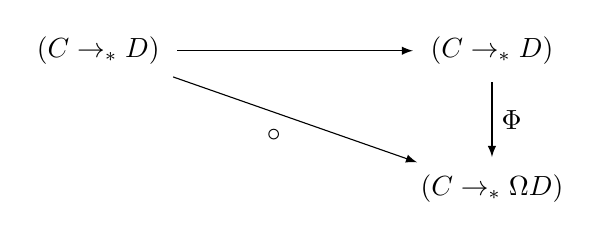
\begin{tikzpicture}[x=5cm,y=-1.75cm,baseline=(current bounding box.center)]
    \tikzset{arrow/.style={shorten >=0.1cm,shorten <=.1cm,-latex}}
    \node (A) at (0,0) {$(C \to_* D)$}; 
    \node (D) at (1,0) {$(\susp C \to_* \susp D)$}; 
    \node (C) at (1,1) {$(C \to_* \Omega \susp D)$}; 
    
    \draw[arrow] (A) to node [above] {$\susp$} (D);
    \draw[arrow] (A) to node [below left] {$\susp \circ \, \blank$} (C);
    \draw[arrow] (D) to node [right] {$\Phi$} (C);
    \end{tikzpicture}
    \end{equation}
\end{lemma}
\begin{proof}
    By easy calculation.
\end{proof}





This equivalence $\Phi$ also satisfies the following lemma:

\begin{lemma} \label{lem:ap-Sigma}
    Let $X$ be a pointed type and $f : A \to B$ be a function.
    The following square commutes (up to homotopy):\todo{check whether it should be $\mathsf{ap}$ or $\Omega(f)$.}
    \begin{equation}
    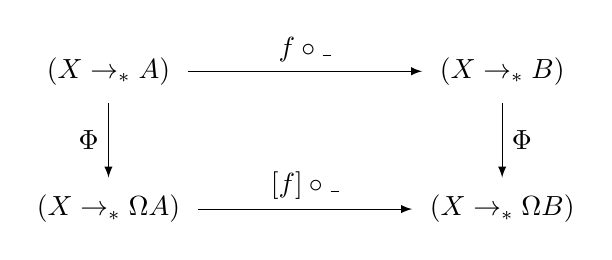
\begin{tikzpicture}[x=5cm,y=-1.75cm,baseline=(current bounding box.center)]
    \tikzset{arrow/.style={shorten >=0.1cm,shorten <=.1cm,-latex}}
    \node (A) at (0,0) {$(\susp X \to_* A)$}; 
    \node (D) at (1,0) {$(\susp X \to_* B)$}; 
    \node (B) at (0,1) {$(X \to_* \Omega A)$}; 
    \node (C) at (1,1) {$(X \to_* \Omega B)$}; 
    
    \draw[arrow] (A) to node [above] {$f \circ \_$} (D);
    \draw[arrow] (A) to node [left] {$\Phi$} (B);
    \draw[arrow] (B) to node [above] {$\ap f \circ \_$} (C);
    \draw[arrow] (D) to node [right] {$\Phi$} (C);
    \end{tikzpicture}
    \end{equation}
\end{lemma}
\begin{proof}
    By calculation.
    %  Starting with $f_0 : \susp X \to A$ and $f_1 : f_0(N) = a_0$ and checking where this pair is mapped if we go first down and then right, we get:
    We start in the top left corner with $g_0 : \susp X \to A$ and $g_1 : g_0(N) = a_0$. If we go first down, then right, we get the following, where we omit the proofs that the functions are pointed:
    \begin{equation}
    \begin{alignedat}{5}
    &\quad && g_0 : \susp X \to A & \\
    \mapsto &&& \lambda x. g_1^{-1} \ct \ap {g_0}(\mathsf{merid}(x) \ct \mathsf{merid}(x_0)^{-1}) \ct g_1 : X \to \Omega A \\
    \mapsto &&& \lambda x. f_1^{-1} \ct \ap {f_0}(g_1)^{-1} \ct  \ap {f_0 \circ g_0}(\mathsf{merid}(x) \ct \mathsf{merid}(x_0)^{-1}) \ct \ap {f_0}(g_1) \ct f_1 : X \to \Omega B
    \end{alignedat}
    \end{equation}
    If we go first right, then down, we get:
    \begin{equation}
    \begin{alignedat}{5}
    &\quad && g_0 : \susp X \to A & \\
    \mapsto &&&  f_0 \circ g_0 : \susp X \to B \\
    \mapsto &&& \lambda x. f_1^{-1} \ct \ap {f_0}(g_1)^{-1} \ct  \ap {f_0 \circ g_0}(\mathsf{merid}(x) \ct \mathsf{merid}(x_0)^{-1}) \ct \ap {f_0}(g_1) \ct f_1 : X \to \Omega B
    \end{alignedat}
    \end{equation}
    The proofs that the functions are pointed are the canonical ones and coincide as well. (todo: if we have a formalisation, we can refer to that.)
\end{proof}

This implies in particular:


\begin{corollary}\label{lem:iterated-ap-Sigma}
    For all $n \geq 0$ and $f$ as above, the diagram
    \begin{equation}
    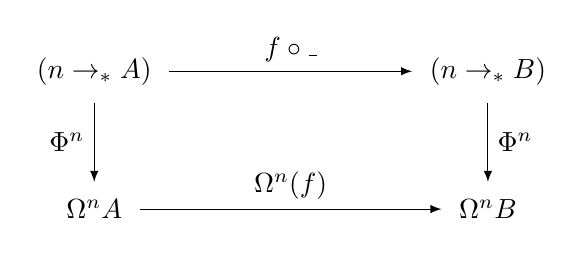
\begin{tikzpicture}[x=5cm,y=-1.75cm,baseline=(current bounding box.center)]
    \tikzset{arrow/.style={shorten >=0.1cm,shorten <=.1cm,-latex}}
    \node (A) at (0,0) {$(\Sn n \to_* A)$}; 
    \node (D) at (1,0) {$(\Sn n \to_* B)$}; 
    \node (B) at (0,1) {$\Omega^n A$}; 
    \node (C) at (1,1) {$\Omega^n B$}; 
    
    \draw[arrow] (A) to node [above] {$f \circ \_$} (D);
    \draw[arrow] (A) to node [left] {$\Phi^n$} (B);
    \draw[arrow] (B) to node [above] {$\Omega^n(f)$} (C);
    \draw[arrow] (D) to node [right] {$\Phi^n$} (C);
    \end{tikzpicture}
    \end{equation}
    commutes.
\end{corollary}
\begin{proof}
    By induction on $n$. Note that $\Sn 0$ is the two-element type,\todo{If we define $\Sn 1 :\equiv \susp(\Sn 0)$ at the very beginning, this is nicer. Maybe say that both are equivalent definitions?} and pointed functions from it into $A$ are determined by a single point in $A$. This makes the case $n \equiv 0$ trivial.
    The step from $n$ to $n+1$ is an application of \cref{lem:ap-Sigma}.
\end{proof}


The above lemmas allow us to formulate a connection between the maps $\susp$ in \eqref{eq:susp-monoid-morphism} and $\sigma$ in \eqref{eq:sigma}:
%, which will be needed in order to use \cref{thm:freudenthal} for \cref{thm:susp-is-monoid-iso}:

\begin{lemma} \label{lem:sigma-susp}
    The maps $\sigma$ and $\susp$ are equal up to canonical isomorphism, i.e.\ the square
    \begin{equation} \label{eq:needs-to-commute}
    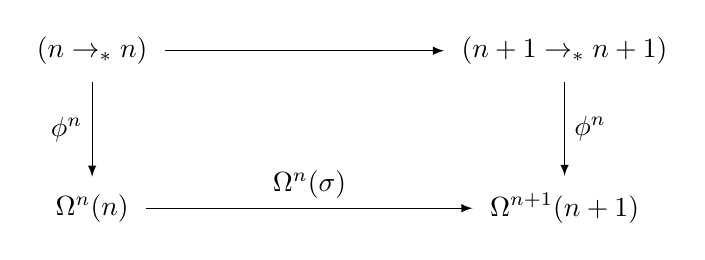
\begin{tikzpicture}[x=6cm,y=-2cm,baseline=(current bounding box.center)]
    \tikzset{arrow/.style={shorten >=0.1cm,shorten <=.1cm,-latex}}
    \node (A) at (0,0) {$(\Sn n \to_* \Sn n)$}; 
    \node (B) at (0,1) {$\Omega^n(\Sn n)$}; 
    \node (C) at (1,1) {$\Omega^{n+1}(\Sn {n+1})$}; 
    \node (D) at (1,0) {$(\Sn {n+1} \to_* \Sn {n+1})$}; 
    
    \draw[arrow] (A) to node [left] {$\phi^n$} (B);
    \draw[arrow] (B) to node [above] {$\Omega^n(\sigma)$} (C);
    \draw[arrow] (D) to node [right] {$\phi^n$} (C);
    \draw[arrow] (A) to node [above] {$\susp$} (D);
    \end{tikzpicture}
    \end{equation}
    commutes.
\end{lemma}
\begin{proof}
 Consider the following:
\begin{equation}
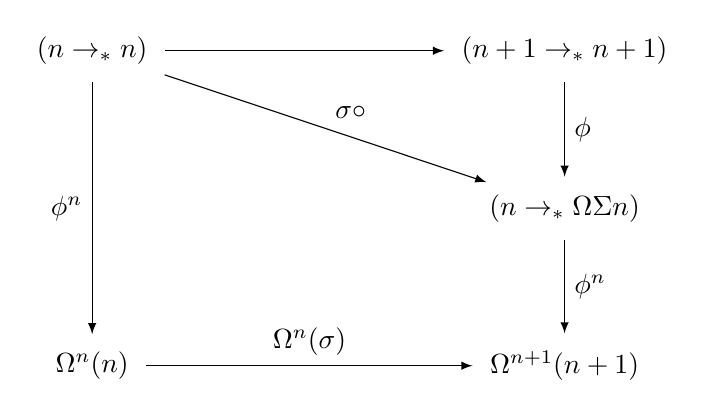
\begin{tikzpicture}[x=6cm,y=-2cm,baseline=(current bounding box.center)]
\tikzset{arrow/.style={shorten >=0.1cm,shorten <=.1cm,-latex}}
\node (A) at (0,0) {$(\Sn n \to_* \Sn n)$}; 
\node (B) at (0,2) {$\Omega^n(\Sn n)$}; 
\node (C) at (1,2) {$\Omega^{n+1}(\Sn {n+1})$}; 
\node (D) at (1,0) {$(\Sn {n+1} \to_* \Sn {n+1})$}; 
\node (E) at (1,1) {$(\Sn n \to_* \Omega \Sigma \Sn n)$};

\draw[arrow] (A) to node [left] {$\phi^n$} (B);
\draw[arrow] (B) to node [above] {$\Omega^n(\sigma)$} (C);
%  \draw[arrow] (D) to node [right] {$\sim$} (C);
\draw[arrow] (A) to node [above] {$\susp$} (D);
\draw[arrow] (D) to node [right] {$\phi$} (E);
\draw[arrow] (E) to node [right] {$\phi^n$} (C);
\draw[arrow] (A) to node [above right] {$\sigma \circ \blank$} (E);
\end{tikzpicture}
\end{equation}
The top triangle commutes by \cref{lem:adj-prop}.
The bottom quadrangle commutes by \cref{lem:iterated-ap-Sigma}.\todo{fix $\ap f$ vs $\Omega(f)$!!}
\end{proof}

\cref{lem:sigma-susp} characterises the function \eqref{eq:susp-monoid-morphism}
in terms of $\sigma$.
Our motivation for this characterisation is that we know something about $\sigma$ through the following result:

\begin{theorem}[{Freudenthal suspension theorem \cite[Thm 8.6.4]{HoTT}}] \label{thm:freudenthal}
    If $X$ is $n$-connected and pointed, with $n \geq 0$, then the map $\sigma$ is $2n$-connected. \qed
\end{theorem}


Choosing $X$ to be $\Sn n$ and using that $\Sn n$ is $(n-1)$-truncated \cite[find-lemma-number]{HoTT}, we get in particular the following instantiation:


\begin{corollary} \label{cor:sigma-truncated}
For $n \geq 1$, the map
\begin{equation} 
\sigma : \Sn n \to \Omega(\Sn {n+1})
\end{equation}
is $2(n-1)$-truncated.
\end{corollary}


To make use of this, we show how connectedness of functions interacts with loop spaces:

\begin{lemma}
    Let $A$ and $B$ be types and $f : A \to B$ be a $k$-connected function ($k \geq -1$).
    For all $a_1, a_2 : A$, the function $\ap f : a_1 = a_2 \to f(a_1) = f(a_2)$ is $(k-1)$-connected.
\end{lemma}
\begin{proof}
    Let us fix $a_1, a_2$, and $p : f(a_1) = f(a_2)$.
    We need to show that the fibre
    \begin{equation}
%        \higherTrunc {k-1} {\Sigma q : a_1 = a_2. \ap{f}(q) = p}
        \Sigma q : a_1 = a_2. \ap{f}(q) = p
    \end{equation}
    is $(k-1)$-connected.
    
%    By the connectedness assumption on $f$, the type $\higherTrunc k {f^{-1}(a_2)}$ is contractible. 
    We consider the two elements 
    $\highertrunc k {(a_1, p)}$ 
    and  
    $\highertrunc k {(a_2, \refl {f(a_2)})}$ of 
    the type $\higherTrunc k {f^{-1}(a_2)}$, which is contractible by the connectedness assumption on $f$.
    Therefore, the type of equalities between the two chosen elements is contractible as well.
    By \cite[Theorem 7.3.12]{HoTT}, this type of equalities is equivalent to
    \begin{equation} \label{eq:eq-in-truncated-fibre}
    \higherTrunc {k-1} {(a_1, p) = (a_2, \refl {f(a_2)})}.
    \end{equation} 
    By \cite[Theorem 2.7.2 and todo-find-number]{HoTT}, 
%    the equality type $(a_1,p) = (a_2,\refl {f(a_2)})$ is 
    this type is further equivalent to
    \begin{equation}
    \higherTrunc {k-1} {\Sigma(q : a_1 = a_2). \ap f(q) = p},
    \end{equation} 
    and the contractibility of this type is exactly what we had to show.
\end{proof}

By $k$-fold application of the above lemma, we get:
\begin{corollary} \label{cor:n-2-connected}
    If $f : A \to_* B$ is $(k+m)$-connected with $k \geq 0$, $m \geq -2$, then
    $\Omega^k(f) : \Omega^k(A) \to \Omega^k(B)$ (viewed as a non-pointed function) is $m$-connected. 
    
    Building on \cref{cor:sigma-truncated} we get that, for $n \geq 1$, the map
    \begin{equation} 
    \sigma : \Omega^n(\Sn n) \to \Omega^{n+1}(\Sn {n+1})
    \end{equation}
    is $(n-2)$-connected.
    \qed
\end{corollary}

We are now ready to restate and prove \cref{thm:susp-is-monoid-iso}:

\suspiso*
\begin{proof}
    Since identity and composition of the monoid structures are just given by the identity function and function composition,
    preservation of the monoid structure is just the (wild) functoriality of $\susp$.
    
    What is left to show is $0$-connectedness.
    In the commuting square of \cref{lem:sigma-susp}, the two vertical maps are equivalences and the bottom horizontal map is $(n-2)$-truncated by \cref{cor:n-2-connected}.
    This implies that the top horizontal map $\susp$ is $(n-2)$-connected as well.
    By assumption we have $(n-2) \geq 0$, which means that an $(n-2)$-connected map is also $0$-truncated.
\end{proof}

Set-truncating a $0$-connected map gives an equivalences, and therefore:
\begin{corollary} \label{cor:iso-of-monoids}
    For all $n \geq 2$, the map
    \begin{equation}
    \higherTrunc 0 {\susp} : \higherTrunc 0 {\Sn n \to_* \Sn n} \to \higherTrunc 0 {\Sn {n+1} \to_* \Sn {n+1}}
    \end{equation}
    is an isomorphism of monoids.\qed
\end{corollary}

Recalling that we eventually want to reach non-pointed equivalences $\Sn n \simeq \Sn n$, 
we want to remove the base points of the monoid morphism above. 
We have the following general result:

\begin{lemma}
    Let $X$ be a type and $x : X$ be a point. If $X$ is connected, then the canonical map which forgets the preservation of the base point $x$, given as
    \begin{alignat}{2}
    \setTrunc{\pi_1}: && \quad & \setTrunc{(X,x) \ptdto (X,x)} \to \setTrunc{X \to X} \\
    &&& \highertrunc 0 {(f,p)} \mapsto \highertrunc 0 f
    \end{alignat}
    is an isomorphism of monoids.
\end{lemma}
\begin{proof}
    We have 
    \begin{alignat}{2}
    &&& \setTrunc{\Sigma(f : X \to X). f(x) = x} \\
    &\simeq &\quad & \setTrunc{\Sigma(f : X \to X). \setTrunc{f(x) = x}} \\
    &\simeq && \setTrunc{X \to X},
    \end{alignat}
    where the first steps holds by \cite[Thm.~7.3.9]{HoTT} and the second by the connectedness assumption.
    Composition and identities are preserved by the projection $\pi_1$, and thus also by $\setTrunc{\pi_1}$.
\end{proof}

Since every $\Sn n$ (for $n \geq 1$) is connected, this allows us to get rid of the preservation of base points in \cref{cor:iso-of-monoids}:

\begin{corollary} \label{cor:higher-spheres-2-comp}
    For all natural numbers $n \geq 2$, the map
    \begin{equation}
    \higherTrunc 0 {\susp} : \higherTrunc 0 {\Sn n \to \Sn n} \to \higherTrunc 0 {\Sn {n+1} \to \Sn {n+1}}
    \end{equation}
    is an isomorphism of monoids.
\end{corollary}

This allows us to see that there are two connected components of symmetries of spheres:

\begin{theorem} \label{thm:higher-spheres-2}
    For any $n \geq 1$, we have an equivalence of type
    \begin{equation}
    \higherTrunc 0 {\Sn n= \Sn n} \weq \bn 2
    \end{equation} 
\end{theorem}
\begin{proof}
    For $n = 1$ and $n=2$, we have established this result in the previous sections (see \cref{todo-enter-thm-numbers}).
    For higher $n$, it follows by induction on $n$ with the help of \cref{cor:higher-spheres-2-comp} that the monoids $\Sn n \to \Sn n$ have exactly two invertible elements.
\end{proof}

\todo[inline]{Nicolai: Now, we can try to show that id and -id are elements of the two components (i.e.\ in different components). I will think about it.}

\section{Appendix}
\label{sec:appendix}



\subsection{Path algebra}
\label{sec:path-algebra}
All through this paper, we deal with pointed functions of the form $f:A \ptdto
\loopspace\null B$. It happens every so often that such an $f$ is pointed by a
path $\refl b = f(a)$ which derives directly from basic path algebra. Because
we use these elementary steps of path algebra in a proof-relevant way, 
we fix names and conventions in this section.

Given a path $p:x=y$ in any type $A$, we denote
\begin{align*}
  \varpi_p &: \refl x = \inv p \refl y p\\
  \omega_p &: \refl x = \inv p p
\end{align*}
Depending on the implementation of concatenation of path, $\omega_p$ and $\varpi_p$
might be definitionally equal. We don't care especially for that, as long at it
is clear that:
\begin{displaymath}
  \varpi_{\refl x} \jdeq \refl {\refl x} \jdeq \omega_{\refl x}  
\end{displaymath}
For any pair of composable paths $p: x=y$ and $q: y=z$, one denotes
\begin{displaymath}
  \kappa_{p,q} : \inv{(qp)} = \inv p \inv q.
\end{displaymath}
Here again, the implementation of $\kappa$ is not important as long as one
makes sure that
\begin{displaymath}
  \kappa_{\refl x,\refl x} \jdeq  \refl {\refl x}
\end{displaymath}

Given a function $f:A\to B$ and $a:A$, the map $\ap f : a=a
\to f(a)=f(a)$ is defined in such a way that $\ap f (\refl a) \jdeq \refl
{f(a)}$. In particular, given an element $b:B$ and a path $p:b=f(a)$, the path
$\varpi_p$ points the map:
\begin{displaymath}
  \loopspace\null (f,p) : \loopspace \null A \to \loopspace\null B, \quad
  q \mapsto \inv p \cdot \ap f(q) \cdot p.
\end{displaymath}
There is also a path witnessing the compatibility of $f$ with concatenation of
paths $p:x=y$ qnd $q:y=z$:
\begin{displaymath}
  \chi_{f,p,q} : \ap f (qp) = \ap f (q) \ap f (p).
\end{displaymath}
Like for the paths $\kappa_{p,q}$, swe are mostly interested in the fact that 
\begin{displaymath}
  \chi_{f,\refl x,\refl x} \jdeq \refl{\refl {f(x)}}.
\end{displaymath}
In the same way there is a witness of the compatibility of $f$ with inversion of
a path $p$:
\begin{displaymath}
  \iota_{f,p} : \ap f(\inv p) = \inv {\ap f (p)}.
\end{displaymath}
This path is defined by induction on $p$ so that $\iota_{f,\refl x} \jdeq
\refl{\refl {f(x)}}$.

Finally, whenever two functions $f:A\to B$ and $g:B\to C$ are composable, there
is, for every path $p$ in $A$, a path $\gamma_{f,g}(p) : \ap{g\circ f}(p) = \ap
g (\ap f (p))$, which is definitionally $\refl{\refl x}$ when $p \jdeq \refl x$.



\subsection{Wild functors}
\label{sec:wild-functors}
The types $\UUptd$ do certainly not form a category {\color{red} of categories???}, 
but some constructions on it are reminiscent of functors. 
\begin{definition}
  A wild functor on $\UUptd$ is a dependent $4$-tuple $(F_0,F_1,c,u)$ where:
  \begin{align*}
    F_0 &:\UUptd \to \UUptd,\\
    F_1 &:\prod_{A,B:\UUptd} (A \ptdto B) \to (F_0(A) \ptdto F_0(B))\\
    c &: \prod_{A,B,C:\UUptd}\prod_{f:A\ptdto B, g:B\ptdto C}F_1(g\circ f) = F_1(g) \circ F_1(f)\\
    u &: \prod_{A:\UUptd} F_1(\id_A) = \id_{F_0(A)}
  \end{align*}
  \label{def:wild-functor}
\end{definition}

As for functors, we usually write both $F_0$ and $ F_1$ only as $F$. The only
relevant fact about $c$ and $u$ is that they exist, 
{\color{red} even though their types are not propositions}. 
Therefore we will often (abusively)
denote a wild functor by its first two components only.

\begin{example}~
  \begin{enumerate}
    \item There is a wild functor $\loopspace \null$ which maps a pointed type $A$
      (pointed at $a$) to $\loopspace \null A \defeq (a=a$)
      (pointed at $\refl a$), and maps
      a pointed function $f: A \ptdto B$ to the pointed function $\loopspace
      \null (f): \loopspace \null A \ptdto \loopspace \null B$ defined as
      follows:
      \begin{displaymath}
        \loopspace \null (f) (p) \defequi \inv{f_0} \cdot \ap f (p) \cdot f_0
      \end{displaymath}
      where $f_0: b=f(a)$ is the path pointing $f$. As noted in
      \cref{sec:path-algebra}, the map $\loopspace \null (f)$ is pointed by the
      path $\varpi_{f_0}:\refl b = \loopspace\null (f)(\refl a)$.
      %
      Whenever $b \jdeq f(a)$ and $f_0 \jdeq \refl {f(a)}$, we have
      $\varpi_{f_0} \jdeq \refl {\refl {f(a)}}$, and in particular, it gives us
      directly the witness $u$ of \cref{def:wild-functor}.
      %
      Moreover, given $f:A \ptdto B$ and $g:B \ptdto C$, one has a path
      $\xi_{f,f_0,g,g_0}(p): \loopspace\null (g\circ f)(p) =
      \loopspace\null(g)(\loopspace\null(f)(p))$ given by a chain of path algebra steps:
      \begin{displaymath}
        \begin{split}
        \xi_{f,f_0,g,g_0}(p) \defequi&
        \ap{\inv {g_0}  \blank g_0}(\inv{\chi_{g,f_0,\inv{f_0}\ap f(p)}})\\
        &\cdot
        \ap{\inv {g_0}  \blank \ap g(f_0) g_0}(\inv{\chi_{g,\ap f(p),\inv{f_0}}})\\
        &\cdot
        \ap{\inv {g_0}  \blank \ap g (\ap f(p)) \ap g(f_0) g_0}(\inv{\iota_{f,f_0}})\\
        &\cdot
        \ap{\inv {g_0} \inv{\ap g(f_0)} \blank \ap g(f_0) g_0}(\gamma_{f,g}(p))\\
        &\cdot
        \ap { \blank \ap{g\circ f}(p) \ap g(f_0) g_0 } (\kappa_{g_0,\ap g (f_0)})
      \end{split}
      \end{displaymath}
      \begin{displaymath}
        \begin{tikzcd}
          \inv{(\ap g(f_0) g_0)} \ap{g\circ f}(p) \ap g(f_0) g_0
          \rar["\kappa"] \ar[ddddr, bend right, dashed]
          & 
          \inv {g_0} \inv{\ap g(f_0)} \ap{g\circ f}(p) \ap g(f_0) g_0 
          \dar["\gamma"]
          \\
          &
          \inv {g_0} \inv{\ap g(f_0)} \ap g(\ap f(p)) \ap g(f_0) g_0 
          \dar["\inv \iota"]
          \\
          &
          \inv {g_0} \ap g(\inv{f_0}) \ap g(\ap f(p)) \ap g(f_0) g_0 
          \dar["\inv \chi"]
          \\
          &
          \inv {g_0} \ap g(\inv{f_0} \ap f(p)) \ap g(f_0) g_0 
          \dar["\inv \chi"]
          \\
          &
          \inv {g_0} \ap g(\inv{f_0} \ap f(p) f_0) g_0 
        \end{tikzcd}
      \end{displaymath}
      The importance thing to notice is that $\xi_{f,\refl {f(a)},g,
      \refl{g(f(a))}}(\refl a) \jdeq \refl {\refl{g(f(a))}}$. Hence, one can
      easily show, by double induction on $p:f(a)=x$ ($x:B$ being a free
      endpoint) and $q:g(x) = y$ ($y:C$ being a free endpoint), that the
      following triangle commutes:   
      \begin{displaymath}
        \begin{tikzcd}
          \loopspace\null (g\circ f)(\refl a) \ar[rr, equal, "\xi_{f,p,g,q}(\refl a)"] 
          \ar[dr, equal, "\varpi_{\ap g(p)q}"swap] & &
          \loopspace\null (g)(\loopspace\null (f)(\refl a)) 
          \ar[dl, equal, "\ap{\loopspace\null(g)}(\varpi_{p})\varpi_{q}"]
          \\
          & \refl c &
        \end{tikzcd}
      \end{displaymath}
      In other words, this provides the witness $c$ of \cref{def:wild-functor}.

    \item There is a wild functor $\susp \null$ which maps a pointed type $A$
      to $\susp A$ (pointed at the pole $N$), and maps a pointed function
      $f:A\ptdto B$ to the pointed function $\susp (f) : \susp A \ptdto \susp
      B$ defined by induction as follows:
      \begin{displaymath}
        \susp (f) (N) \defequi N,\quad
        \susp (f) (S) \defequi S,\quad
        \ap{\susp (f)} \circ \mrd = \mrd \circ f.
      \end{displaymath}
      Note that $\susp (f)$ is pointed by definition as it maps $N$ to $N$
      directly. The witnesses $u$ and $c$ of \cref{def:wild-functor} are
      straightforward through degenerate induction on the supsension.
  \end{enumerate}
\end{example}

\begin{definition}
  Given two wild functors $L$ and $R$, a wild adjunction of type $L\leftadjto
  R$ is a dependent function $\Phi$ that maps pointed types $A,B:\UUptd$
  to an element
  \begin{displaymath}
    \Phi_{A,B} : (LA\ptdto B) \weq (A\ptdto RB)
  \end{displaymath}
  such that $\Phi_{A,B}(\blank) \circ f = \Phi_{A',B} (\blank \circ L(f))$ for
  any $f:A'\ptdto A$ and $\Phi_{A,B'}(g\circ\blank) = R(g)\circ \Phi_{A,B}
  (\blank)$ for any $g:B\ptdto B'$.
  \label{def:wild-adj}
\end{definition}

\begin{proposition}
  There is a wild adjunction $\susp \null \leftadjto \loopspace \null$.
  \label{prop:susp-loop-adjunction}
\end{proposition}
\begin{proof}
  Let $A$ and $B$ be pointed types, with respective distinguished point $a$ and
  $b$. Given $f:\susp A \ptdto B$ pointed by $f_0:b = f(N)$, define for every
  $x:A$
  \begin{displaymath}
    \Phi_{A,B}(f) (x) \defequi \inv{f_0} \cdot \ap f (\inv{\mrd(a)}\mrd(x)) \cdot f_0
  \end{displaymath}
  This function $\Phi_{A,B}(f): A \to \loopspace\null B$ is pointed by path algebra
  \begin{displaymath}
    \ap{\inv{f_0} \ap f(\blank) f_0 }(\omega_{\mrd(a)}) \cdot \varpi_{f_0} 
  \end{displaymath}
  
  The function $\Phi_{A,B}$ is an equivalence: indeed define a pseudo-inverse
  $\Psi_{A,B}$ as the function that maps $f: A\ptdto \loopspace\null B$ to the
  pointed map $\susp A \ptdto B$ defined by induction through 
  \begin{displaymath}
    \Psi_{A,B}(f)(N) \defequi b,\quad \Psi_{A,B}(f)(S) \defequi b,\quad
    \ap{\Psi_{A,B}(f)}\circ\mrd = f.
  \end{displaymath}
  The function $\Psi_{A,B}(f)$ is pointed by $\refl b$. For future references,
  denote $\mu$ for the path $\ap{\Psi_{A,B}(f)}\circ \mrd = f$.
  
  Let us first show that $\Phi_{A,B}(\Psi_{A,B}(f)) = f$ for any pointed map $f:A\to
  \loopspace\null B$. Let us denote $f_0: \refl b = f(a)$ the path pointing
  $f$. The function $\Phi_{A,B}(\Psi_{A,B}(f))$ maps $x:A$ to 
  \begin{displaymath}
    \refl b\cdot \ap{\Psi_{A,B}(f)}(\inv{\mrd(a)}\mrd(x))\cdot \refl b
  \end{displaymath}
  There is a path $p_x$ from this element to $f(x)$ obtained by composing all the
  following paths ({\color{red} Drawing? diagrams?}):
  \begin{align*}
    \ap{\refl b \cdot \blank \cdot \refl b}(\chi_{\Psi_{A,B}(f),\inv{\mrd(a)},\mrd(x)}),
    \\
    \ap{\refl b \cdot \ap{\Psi_{A,B}(f)}(\inv{\mrd(a)}) \cdot \blank \cdot \refl b}(\mu(x)),
    \\
    \ap{\refl b \cdot \blank \cdot f(x) \cdot \refl b}(\iota_{\Psi_{A,B}(f),\mrd(a)}),
    \\
    \ap{\refl b \cdot \blank \cdot f(x) \cdot \refl b}(\ap{\inv\blank}(\mu(a))),
    \\
    \ap{\refl b \cdot \blank \cdot f(x) \cdot \refl b}(\ap{\inv\blank}(f_0)),
    \\
    \tau_{f(x)}
  \end{align*}
  ({\color{red} add a path in beginning of appendix $\tau_p: \refl x p \refl x
  = p$ that also satisfies $\tau_{\refl x} \jdeq \refl{\refl x}$}).

  To finish proving that $\Phi_{A,B}(\Psi_{A,B}(f)) = f$, one shall now prove
  that the transport of the path pointing $\Phi_{A,B}(\Psi_{A,B}(f))$ over $p$
  is equal to $f_0$. In other words, we want the following triangle to commute:
  \begin{displaymath}
    \begin{tikzcd}
      \Phi_{A,B}(\Psi_{A,B}(f)) (a) \rar[equal, "p_a"] 
      \drar[equal, "\ap{\refl b\cdot \ap{\Psi_{A,B}(f)}(\blank) \cdot \refl b}(\omega_{\mrd(a)}", swap]
      & f(a) \dar[equal, "f_0"]
      \\
      & \refl b 
    \end{tikzcd}
  \end{displaymath}
  {\color{red}This is true, basically just astract properties of $\omega$ against application of functions + little induction. Yet TODO properly!}  

  We continue by showing giving an element of $\Psi_{A,B}(\Phi_{A,B}(f)) = f$
  for any pointed map $f: \susp A \ptdto B$, where the path of $f$ is denoted
  $f_0:b = f(N)$.  First let us give an element $p_f$ of
  $\Psi_{A,B}(\Phi_{A,B}(f)) = f$ as (unpointed) functions, by induction on $\susp A$ by
  providing: 
  \begin{enumerate}
    \item the path $f_0:\Psi_{A,B}(\Phi_{A,B}(f))(N) \jdeq b = f(N)$,
    \item the path $\ap f(\mrd(a))\cdot f_0:\Psi_{A,B}(\Phi_{A,B}(f))(S) \jdeq b = f(S)$.
  \end{enumerate}
  All we need is now a path over $\pathover {f_0} {T}{\mrd(x)} {\ap f{\mrd(a)} \cdot
  f_0}$ for any $x:A$, where $T$ is the type family $(y:\susp A) \mapsto
  \Psi_{A,B}(\Phi_{A,B}(f))(y) = f(y)$. In other words, for any $x:A$, one
  wants to provide a witness for the commutativity of the following square:
  \begin{displaymath}
    \begin{tikzcd}[column sep=large]
      b \dar["\inv{f_0}\ap f(\inv{\mrd(a)}\mrd(x)) f_0"swap] \rar["f_0"] 
      & f(N) \dar["\ap f (\mrd(x))"]
      \\
      b \rar["\ap f (\mrd(a))f_0"swap] & f(S)
    \end{tikzcd}
  \end{displaymath}
  The witness is simply provided by path algebra. The last bit of information
  to provide is the compatibility of $p_f$ with the paths pointing
  $\Psi_{A,B}(\Phi_{A,B}(f))$ and $f$: we must show that $p_f(N) \cdot refl b =
  f_0$. This is immediate as we defined $p_f(N)$ to be $f_0$ definitionally.

  It remains to prove that the equivalence $\Phi_{A,B}$ is natural in $A$ and
  $B$ in the sense of \cref{def:wild-adj}.
\end{proof}


\subsection{Old section: Symmetries of the $n$-Sphere}

\todo[inline]{Nicolai: I have replaced the $n\geq 2$ development with my completed approach. I keep the old attempt here, it contains a few ideas which I have not used but which could still be of interest.}

In this section, we want to generalize the work done on the $2$-sphere to higher
spheres. More precisely, we will prove that
\begin{theorem}
    \label{thm:higher-spheres}
    For all $n\geq 1$, $\setTrunc{\Sn n = \Sn n} \weq \bn 2$.
\end{theorem}

If we manage to prove that $\id_{\Sn n}$ is not merely equal to $-\id_{\Sn n}$,
then together with \cref{prop:sups-components-are-equiv}, one has the slightly
better result:
\begin{displaymath}
(\Sn n = \Sn n) \weq \bn 2 \times \conncomp{(\Sn n = \Sn n)}{\id_{\Sn n}}
\end{displaymath}
{\color{red} Maybe add a remark as: This is reminiscent of the well-know result
    about the orthogonal group: $\mathrm O(n)$ is a Lie group with 2 connected
    components, both diffeomorphic to $\mathrm{SO}(n)$.
}
%

\cref{sec:sphere} provides the base case for a proof by induction on $n \geq 2$
of \cref{thm:higher-spheres}. We will now focus on the induction step. 
%
We take an interest in the following map, induced by the suspension wild functor:
\begin{displaymath}
\susp (\blank) : (\Sn n \ptdto \Sn n) \to (\Sn {n+1} \ptdto \Sn{n+1})
\end{displaymath}
The wild nature of the functor just vanishes once the function types are
set-truncated.
%
In other words, it means that the following map is a morphism of monoids:
\begin{displaymath}
\setTrunc{\susp(\blank)} : \setTrunc{\Sn n \ptdto \Sn n} \to \setTrunc{\Sn {n+1} \ptdto \Sn{n+1}}
\end{displaymath}

\begin{proposition}
    For $n\geq 2$, $\setTrunc{\susp(\blank)}$ is an isomorphism of monoids.
    \label{prop:susp-iso-monoids}
\end{proposition}
\begin{proof}
    {\color{red}Freudenthal + check Marc's diagram.}
\end{proof}

\begin{lemma}
    Let $A$ be a pointed type. The type of invertible elements in the monoid $\setTrunc{A \ptdto A}$
    is the (essential) image of the induced inclusion $i:\setTrunc{A \ptdweq A} \to
    \setTrunc{A \ptdto A}$.
    \label{lemma:invertible-truncated-Sn-pointed-weq}
\end{lemma}
\begin{proof}
    Obviously, the truncation $\settrunc{f}$ of an equivalence $f$ is invertible,
    as $\settrunc{\inv f}$ is an inverse for it.
    
    Conversely, if $x:\setTrunc{A \ptdto A}$ is invertible, then 
    it has a unique inverse $\inv x$, and we want to
    produce an element of the type:
    \begin{displaymath}
    \sum_{y:\setTrunc{A \ptdweq A}} x = i(y)
    \end{displaymath}
    %
    As $x=i(y)$ is a proposition for every $y$ in the set $\setTrunc{A
        \ptdweq A}$, this type is a set itself. Hence, one might assume
    that $x \jdeq \settrunc f$ for some function $f:A \ptdto A$ as well
    as its inverse $\inv x \jdeq \settrunc g$ for some $g:A \ptdto A$. 
    %
    From the inverse law in the monoid $\setTrunc{A \ptdto A}$, one
    derives that both $fg$ and $gf$ are merely equal to $\id_{A}$. To prove
    the proposition that $f$ is an equivalence, on can then assume actual
    witnesses of $fg=\id_{A}$ and $gf=\id_{A}$. Then $g$ is a
    pseudo-inverse for $f$, which solves the problem.
\end{proof}

\begin{corollary}
    For any $n\geq 2$, $\setTrunc{\Sn n \ptdweq \Sn n} \weq \bn 2$.
    \label{cor:Sn-pointed-weq-is-bool}
\end{corollary}
\begin{proof}
    We have shown the result for $n=2$ in the previous chapter
    (\cref{cor:equivalence-conn-component}). Suppose $n\geq 2$. By
    \cref{prop:susp-iso-monoids}, the monoids $\setTrunc{\Sn n \ptdto \Sn n}$ and
    $\setTrunc{\Sn {n+1} \ptdto \Sn {n+1}}$ are equivalent. Hence, their respective
    submonoids of invertible elements are also equivalent. By
    \cref{lemma:invertible-truncated-Sn-pointed-weq}, the type $\setTrunc{\Sn n
        \ptdweq \Sn n}$ is then equivalent to $\setTrunc{\Sn {n+1} \ptdweq \Sn
        {n+1}}$.
    
    The result is then proved by induction on $n\geq 2$.
\end{proof}

To prove \cref{thm:higher-spheres}, we need to get from this result to {\em
    unpointed} equivalences. For the next lemma, consider $\Sn n$ as a bare type
and let us use $(\Sn n,x)$ to mean the type $\Sn n$ pointed by an element
$x:\Sn n$.
\begin{lemma}
    Let $n\geq 2$. For all $x:\Sn n$, one has $\setTrunc{(\Sn n, N) \ptdweq (\Sn n, x)} \simeq \bn 2$.
    \label{lemma:pointed-weq-free-point-codomain-is-bool}
\end{lemma}
\begin{proof}
    The type $P(x) \defequi \setTrunc{(\Sn n, N) \ptdweq (\Sn n, x)} \simeq \bn 2$ is a
    set, i.e.\ $0$-truncated.
    Further, the sphere $\Sn n$ is $(n-1)$-connected and the map $1\to \Sn n$ selecting the point $N$ is therefore
    $(n-2)$-connected. 
    By \cite[Lemma 7.5.7]{HoTT} and by the assumption $n \geq 2$,
    it suffices to give an element of $P(N)$ to get a
    dependent function in $\prod_{x:\Sn n}P(x)$. This element of $P(N)$ is
    provided by \cref{cor:Sn-pointed-weq-is-bool}.
\end{proof}

We can now give a proof of \cref{thm:higher-spheres}.
\begin{proof}[Proof of \cref{thm:higher-spheres}]
    One relies on the well-know equivalence:
    \begin{displaymath}
    (\Sn n \weq \Sn n) = \sum_{x:\Sn n}\left( (\Sn n, N) \ptdweq (\Sn n, x) \right)
    \end{displaymath}
    By \cite[Thm 7.3.9]{HoTT}, the $k$-truncation of a total space
    $\sum_{x:A}P(x)$ is equivalent to the $k$-truncation of the space
    $\sum_{x:A}\Trunc{P(x)}_k$. Hence, we find:
    \begin{align*}
    \setTrunc{\Sn n = \Sn n} &\weq \setTrunc{\Sn n \weq \Sn n} \\
    &\weq \setTrunc{\sum_{x:\Sn n} (\Sn n, N) \weq (\Sn n, x)} \\
    &\weq \setTrunc{\sum_{x:\Sn n} \setTrunc{(\Sn n, N) \weq (\Sn n, x)}} \\
    &\weq \setTrunc{\Sn n \times \bn 2} \\
    &\weq \setTrunc{\Sn n} \times \setTrunc{\bn 2} \\
    &\weq \bn 2
    \end{align*}
\end{proof}


\bibliographystyle{alpha}
\bibliography{bib}

\end{document}


%%% Local Variables:
%%% mode: latex
%%% TeX-master: t
%%% reftex-default-bibliography: ("bib.bib")
%%% End:
